\subsection{Clustering the resource graph}
\label{sec:gener-reso-graph}

The resource graph represents the cluster of compute nodes on which the
filter graph will be executed. % There is a plethora of different
% architectures and topologies that an HPC architecture might be
% configured in. Hence, in order to accommodate the varying types of
% topologies and configurations, we use synthetic topologies to test our
% partitioning framework.
A sample resource graph is shown in Figure~\ref{fig:res} at level 0. The
resource graph that is shown is heterogeneous in both computation and
communication. The properties of the resource graph are described below:

\begin{itemize}

\item \textbf{Compute nodes:} The compute nodes (PEs) are assumed to
  belong under two categories of processing units, mainly CPUs and
  GPUs. Following the current trend, the CPUs have a larger MIPS
  count. The MIPS capacity of a PE is denoted by the first constraint
  $R^i_0, \forall i \in V_r$. The GPU nodes have a lower MIPS count, but
  have a large vector length, denoted by the second constraint
  $R^i_1, \forall i \in V_r$. For example, the fifth PE (\texttt{E0}) at
  level 0 is a CPU, since it has a small vector count and a large MIPS
  count, the first PE (\texttt{A0}) on the other hand is a GPU, since
  the capabilities are reversed.

  % The scalar instructions of a Processing Element (\textbf{PE}) that
  % represents a CPU is much higher that that of a GPU. At the same time
  % parallel vector operations that a \textbf{PE} representing a GPU is
  % much higher compared to that of a CPU. In Fig \ref{fig:res} $ R^1 $ is
  % a 'CPU' and $ R^5 $ is a 'GPU'.

\item \textbf{Communication links:} The resource graph shown in
  Figure~\ref{fig:res} at level 0, follows a 2D mesh topology. In this
  topology the PEs are connected in a grid with individual communication
  links between them. The bandwidth of these links is non uniform. The
  different bandwidths on the communication links is represented by the
  constraint $E^C$. Our framework can handle any kind of topology, the
  2D mesh shown in Figure~\ref{fig:res}, is just an example topology.

\end{itemize}

\subsubsection{Clustering the topology}
\label{sec:clustering-topology}

% Mapping the filter graph on a heterogeneous architecture is a known NP
% hard problem. The problem mainly lies in the size of the resource
% graph and the sheer number of ways in which the filter graph can be
% mapped on to the resource graph. In our approach we take a staged
% graph partitioning approach.
The \underline{main idea} behind our partitioning approach is to first
hierarchically cluster the nodes in the heterogeneous architecture provided
by the designer, thereby forming clusters. The
application is then partitioned in stages (levels) onto the resulting
hierarchy. The \underline{intuition} behind this approach is two fold:

\begin{itemize}

\item \textit{Heterogeneous K-way partitioning:} The process of
  partitioning an application onto a given architecture is equivalent to
  a heterogeneous K-way partitioning problem. Hierarchically clustering
  a heterogeneous topology such that the resulting hierarchy consists of
  clustered PEs with balanced compute capabilities can reduce the
  heterogeneous K-way partitioning problem to a homogeneous one.

\item \textit{Considering communication links:} The communication can be
  considered into the equation, while building the hierarchical cluster
  using the min-cut technique. Thus, a min-cut load-balancing of the PEs
  in a topology intuitively means: we are clustering together PEs, which
  have large bandwidth together into a single cluster, while
  making an attempt to load balance the two capabilities: MIPS and
  vector lengths.

\end{itemize}

The hierarchical cluster built for the synthetic topology at level 0 of
Figure~\ref{fig:res}, is shown in the levels 1-3. The stages used to
build the hierarchy are as follows:

\begin{itemize}

\item \textit{Effective computation during clustering:} Given a
  topology graph with $|V_r|$ resources, we cluster the PEs in levels,
  whereby the height of the cluster is $log_2|V_r|$. For example,
  consider the PEs at level 0 in Figure~\ref{fig:res}. Clustering from
  level 0 to level 1 results in 4 PEs at level 1, where the two
  capabilities, $R^k_0,\ R^k_1$ for each cluster $k = \{i, j\},
  \exists i \in V_r \wedge \exists j \in V_r$ is computed as: $R^k_0 =
  R^i_0 + R^j_0$, and $R^k_1 = R^k_1 + R^j_1$. Without loss of
  generality we assume this for any $k = \{i,j,..,n\}, \forall n \in
  V_r$. This process is continued until we reach the top-level with just
  1 cluster. We end up with a load-balanced hierarchy, with each
  level showing a larger amount of homogeneity, and a smaller number of
  clustered PEs. The reason for a level based clustering, instead of
  clustering all nodes into a single 2 node partition, is that when
  partitioning the application on the resulting top-down cluster, we
  have fine grained details within each of the cluster.

  % \item Firstly, we form virtual representations of the resource graph
  %   by clustering the nodes. These virtual nodes are formed by min
  %   cutting communication volume and load balancing the virtual nodes
  %   capabilities.  The formation of these virtual nodes creates
  %   homogeneous partitions from hetrogeneous PEs.

  % \item Secondly, instead of doing this in a single step, we construct
  %   this in several level by clustering half the nodes from the
  %   previous level. We end up with a structure consisting of several
  %   levels, where the $ Number\ of\ levels = log_2 ( Number\ of\ Nodes
  %   )$.

\item \textit{Effective communication during clustering:}
  When clustering nodes the effective communication between two such clusters is
  hard to determine. This is because the clustering itself is a virtual
  representation of the actual nodes. Moreover there might be multiple unique 
  paths between two nodes across different clusters. Choosing a suitable path 
  is a routing problem and its beyond the scope of this paper.

  Instead we assume that in the worst case scenario the link with the least 
  bandwidth would act as the bottleneck. These unique links are determined
  for all the nodes in the cluster. Then to get the \textit{effective
  bandwidth} between these clusters we aggregate these bandiwdths.
  The various steps in which this is calculated is explained below:

  \begin{enumerate}

  \item We use the all-pair Floyd-Warshall~\cite{sski08} algorithm to calculate
  the shortest path, in terms of latency of data-transfer, for every
  communication link in the topology. From this we calculate the bandwidth of
  these links by inverting its latency. This creates a list which contains all
  of the best case bandwidth between any two nodes.

  \item For any two clusters, we assume a source node in one cluster and
  determine the paths to all the nodes across the cluster. From this we choose
  the link with the least bandwidth.

  \item Then we repeat the step above for the other nodes and end up with the
  paths which would act as a bottleneck for any given unique source and
  destination pair.

  \item On aggregating the bandiwdths of all these links we end up with the
  effective bandiwdth between the two clusters.

  \end{enumerate}

  The purpose of calculating this effective bandwidth is that during clustering
  of the nodes at each level we would like to balance the nodes not only based on
  their compute capabilities but also their communication potential. This would
  give us more balanced clusters with both computation and communication taken
  into account.

  %~ There are a number of paths that communication between two
  %~ nodes might follow. The \underline{effective bandwidth} between any
  %~ two nodes in different cluster depends upon the route in the topology graph
  %~ between these contracted nodes.
%~
%~
   %~ Once the nodes are contracted we use the bottleneck
  %~ amongst these possible links as our effective bandwidth.

  For the topology, at level 0, in Figure~\ref{fig:res}, we first
  calculate the best possible paths between every pair of nodes
  \mbox{$(i,j) \in (V_r \times V_r)$}. Now let us consider the example
  of the clustered nodes \texttt{B1} and \texttt{C1}. Node \texttt{B1}
  is a cluster of the set of children nodes $\{3, 8, 6\}$ and
  \texttt{C1} is the cluster of the node set $\{2, 1\}$. Being an
  undirected graph with loss of generality we can consider \texttt{B1}
  to be the source and \texttt{C1} to be the destination. Hence, the
  worst path, in terms of latency of data-transfer, following the
  all-pair Floyd-Warshall algorithm, between nodes $3$ and $2$ within
  the clustered nodes is given by the maximum latency path amongst the
  memoized best edges: $max((3,2),\ (8,2),\ (6,2))$. Similar computation
  is carried out for all link pairs in the clustered node with $1$ as
  the destination node to find the minimum latency path. Finally, the
  reciprocal of these two latencies and its addition gives us the
  effective bandwidth between the two clusters. This effective
  bandwidth represents the communication link between the two clustered nodes.

  % The communication bandwidth between the clustered nodes is determined
  % by,\\ ${ \sum ( \min for same destn ( \max bw R^i, R^j ) ) ) }$\\ The
  % max bandiwdths between any ${R^i}$ is determined by floyd warshall
  % algorithm.

% \item The capabity of each of the PEs that are clustered together are
% aggregated to form the larger virtual node.

% \item In each level PEs with high communication bandwidth and balanced
% capabilities are clustered together. In doing this in a bottom up
% approach i.e. clustering instead of partitioning, we allow the nodes to
% form without ignoring communication links between the nodes. This also
% avoids the formation of dangling nodes in the graph.

\end{itemize}

\begin{figure}[ht]
  % \centering
  \includegraphics[scale=0.43]{./figures/resource}
  \caption{Clustering of a resource graph}
  \label{fig:res}
\end{figure}

% \begin{figure*}[ht!]
%   \centering
%   % 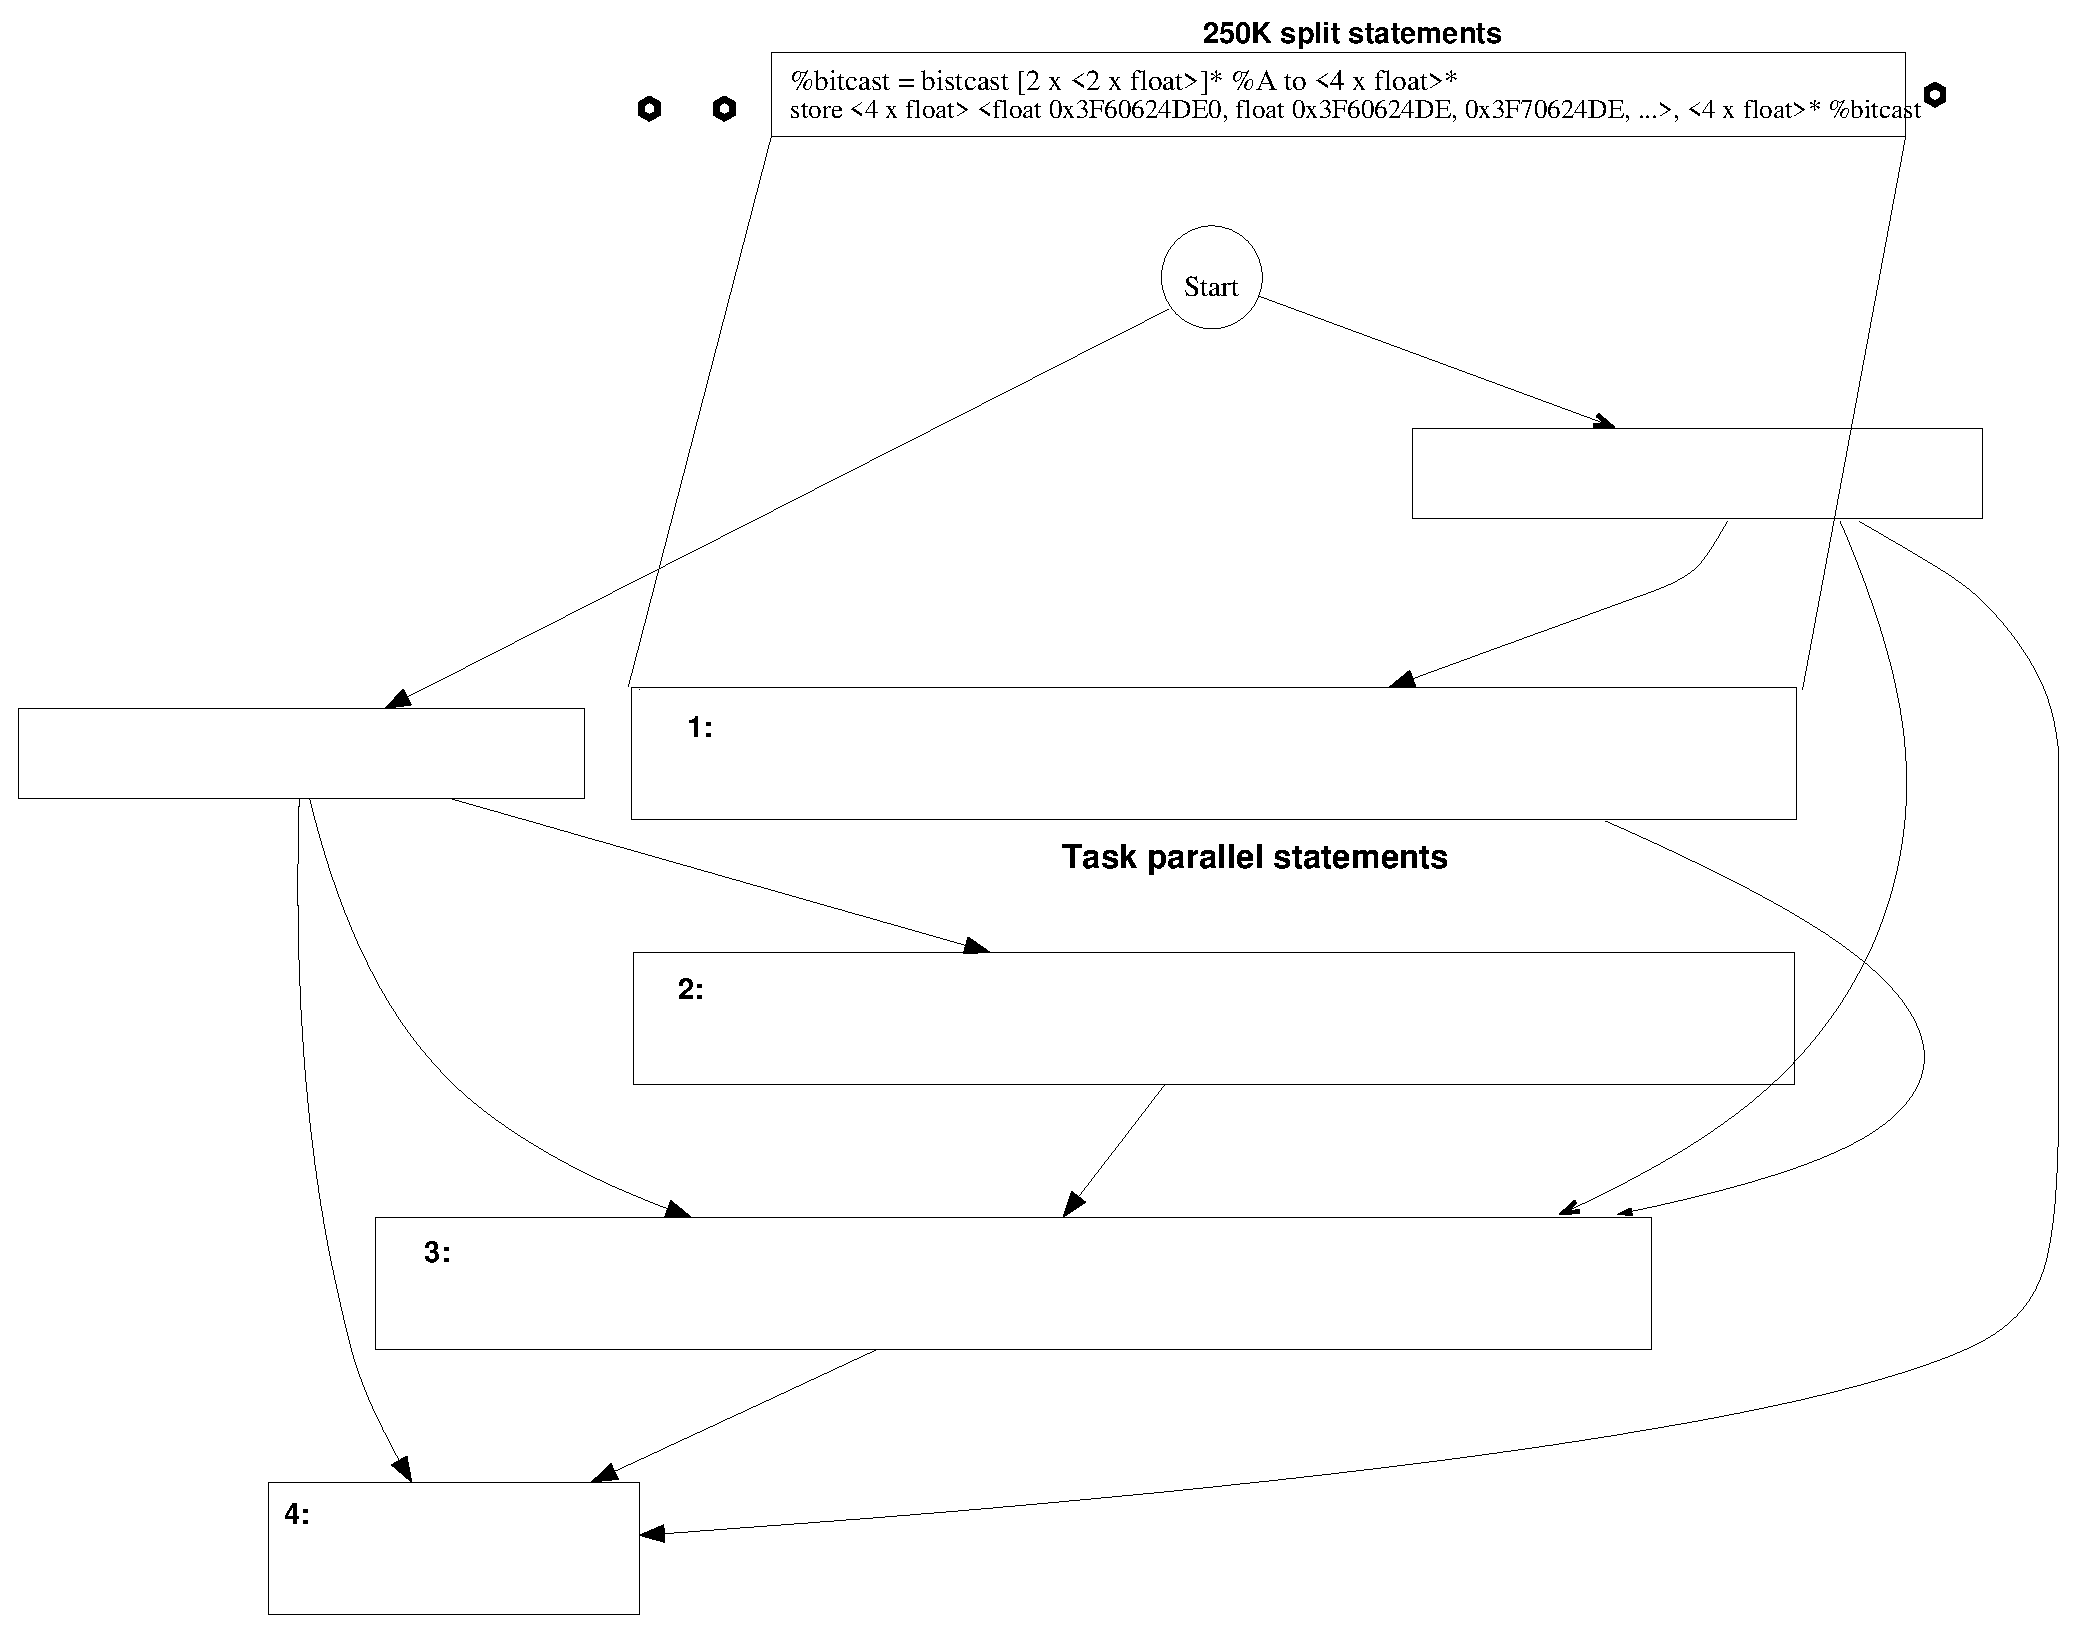
\includegraphics[scale=0.42]{./figures/jacobi2d}
%   \scalebox{0.4}{\input{./figures/dendrogram.pstex_t}}
%   \caption{The dendrogram for Figure~\ref{fig:res}}
%   \label{fig:7}
% \end{figure*}

% In fig \ref{fig:res} we show our clustering approach on a 4x2 mesh. At
% each level suitable nodes are clustered together to form a larger node.
% We see that the PE $ R^3 $ and PE $ R^8 $ are combined together
% when moving from level 0 to level 1. Overall, we reach three levels
% and at the top most level all the nodes from a single virtual node.

\subsection{Task graph partitioning}
\label{sec:filter-graph-part}

The filter partitioning on the resulting hierarchical cluster takes a
top-down approach. We start with the filter graph extracted from the
application (Figure~\ref{fig:1}). We then recursively partition the filter
graph (using K-way partitioning) on the hierarchical cluster of the
resource-graph. For the example cluster in Figure~\ref{fig:res}, we
start by partitioning the filter graph in Figure~\ref{fig:1}, first into
two (K=2) partitions considering two equally weighted compute nodes at
level 2. Once a partition is obtained for this level, we move onto the
next level (level 1), whereby all the filter graph nodes allocated onto
node \texttt{A2} are further partitioned onto the nodes \texttt{A1} and
\texttt{C1} (again K=2), which are coupled into the cluster
\texttt{A2}. This process is continued recursively for all clusters until the
final level (level 0). During each partition we make
sure that the filter node requirements are closely matched to the resource
node capabilities.

% To partition the application we start with the top most level in the
% resource graph and divide it according to the required virtual nodes at
% that level. We then move on to the next level and partition the
% application on to the virtual nodes that the current node belongs to.
% In this way we follow the structure of the resource graph until we reach
% level, by which reach the actual mapping of the filter graph on to the
% resource graph.

Doing it in this top down manner has two important consequences.

\begin{itemize}

\item \textit{Increase in the time complexity:} As stated previously,
  the partitioning problem is equivalent to the K-way partitioning
  problem. The multi-level K-way partitioning results in the worst cast
  time complexity of $O(|E_t| \times log_2|V_r|)$~\cite{gkar98}. Our
  algorithm gives a worst case complexity of \mbox{$log_2|V_r| \times
    O(|E_t| \times log_2 |V_r|)$} when using the multi-level K-way
  partitioning. But, in the average case we ask for a balanced 2-way
  partition at all levels, which results in a complexity of $log_2 |V_r|
  \times O (E_t)$ in the average case.

\item \textit{Refined mapping:} By dividing the mapping on to several
  levels we can achieve much better load balancing by considering only
  fewer nodes to map than if we were to do it directly on to the
  resource graph. % We show this quantitatively in the Experimental
  % results section~\ref{sec:experiments-results}.

\end{itemize}


%%% Local Variables:
%%% mode: latex
%%% TeX-master: "bare_conf"
%%% End:
